\chapter{Background}

This chapter provides the necessary background for the denoising methods explored in this work.
We begin by defining the general denoising problem and discussing its inherent challenges.
We then introduce distributed acoustic sensing (DAS) as a real-world application and highlight the unique difficulties it poses.
Finally, we present key deep learning concepts and techniques that are used in the context of denoising.

\section{Denoising}\label{sec:denoising}

In general, denoising refers to the process of recovering a clean signal from a noisy observation.
Formally, this is described by the inverse problem 
\begin{equation}
    y = x + n
\end{equation}
where $y$ is the noisy observation, $x$ is the underlying clean signal and $n$ represents some form of noise, for example Gaussian noise~$n \sim \normal$.
Since both the noise and its distribution are often unknown, denoising is an inherently ill-posed problem, as multiple solutions can explain the same noisy data.
Therefore, additional assumptions or constraints on the solution space are necessary, a process typically referred to as regularization.
This can involve the use of a \textit{prior}, which encodes our beliefs about the likely properties of the clean signal.
The choice of regularizer or prior depends on the specific problem setting and the type of data involved.

\section{Distributed Acoustic Sensing}

Distributed acoustic sensing (DAS), also known as distributed vibration sensing (DVS)~\cite{DAS}, is an innovative technology for high-resolution vibration measurements over large distances by utilizing fiber optic cables as sensor arrays.
When a short laser pulse is sent through the fiber by a DAS interrogator unit, a fraction of the light is scattered back due to small variations or imperfections in the fiber.
This phenomenon is referred to as Rayleigh scattering.
\begin{wrapfigure}{r}{0.48\textwidth}
    \centering
    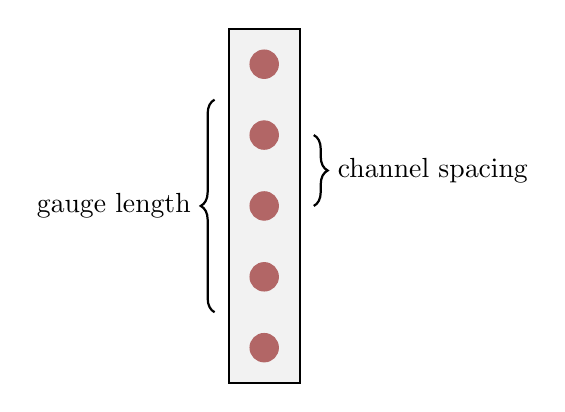
\begin{tikzpicture}[scale=0.9]
        \filldraw[color=gray!10,draw=black,thick] (0,0) -- (1,0) -- (1,5) -- (0,5) -- cycle;        \foreach \i in {0,1,2,3,4} {
            \filldraw[color=Maroon!60] (0.5,\i+0.5) circle (0.2); 
        }

        \draw[decorate,decoration={brace,amplitude=5pt}, thick] (-0.2,1) -- (-0.2,4);
        \draw[decorate,decoration={brace,amplitude=5pt}, thick] (1.2,3.5) -- (1.2,2.5);

        \node at (-0.4,2.5) [left] {gauge length};
        \node at (1.4,3) [right] {channel spacing};
    \end{tikzpicture}

    \caption{
        Gauge length and channel spacing. Red dots represent the individual channels along the fiber.
        Figure adapted from~\cite{GaugeLength}.
    }\label{fig:gauge-length}
\end{wrapfigure}
Vibrations along the cable caused by external influences, e.g.\ seismic events, strain the fiber, which in turn causes phase shifts in the backscattered light.
These shifts are detected by the interrogator and, since the travel time of the light is known, can be used to accurately locate the strain along the cable~\cite{DAS-N2N}.
In order to extract meaningful measurements, strain is analyzed over sections of the fiber, rather than at individual points.
The length of these sections is called the gauge length, while another parameter, the channel spacing, determines how much this section is moved for each measurement, or channel, along the cable~\cite{GaugeLength}.
In practice, each channel corresponds to a virtual sensor capturing the average strain within its gauge length.
Typically, the gauge length is selected to be bigger than the channel spacing, meaning that the measurement sections of neighboring channels overlap, as visualized in Figure~\ref{fig:gauge-length}.
This concept of virtual sensors leads to high cost-effectiveness and, paired with the high sample rates enabled by the optical approach, allows measurements with significantly higher spatial and temporal resolution compared to conventional seismographs.

\begin{figure}[b!]
    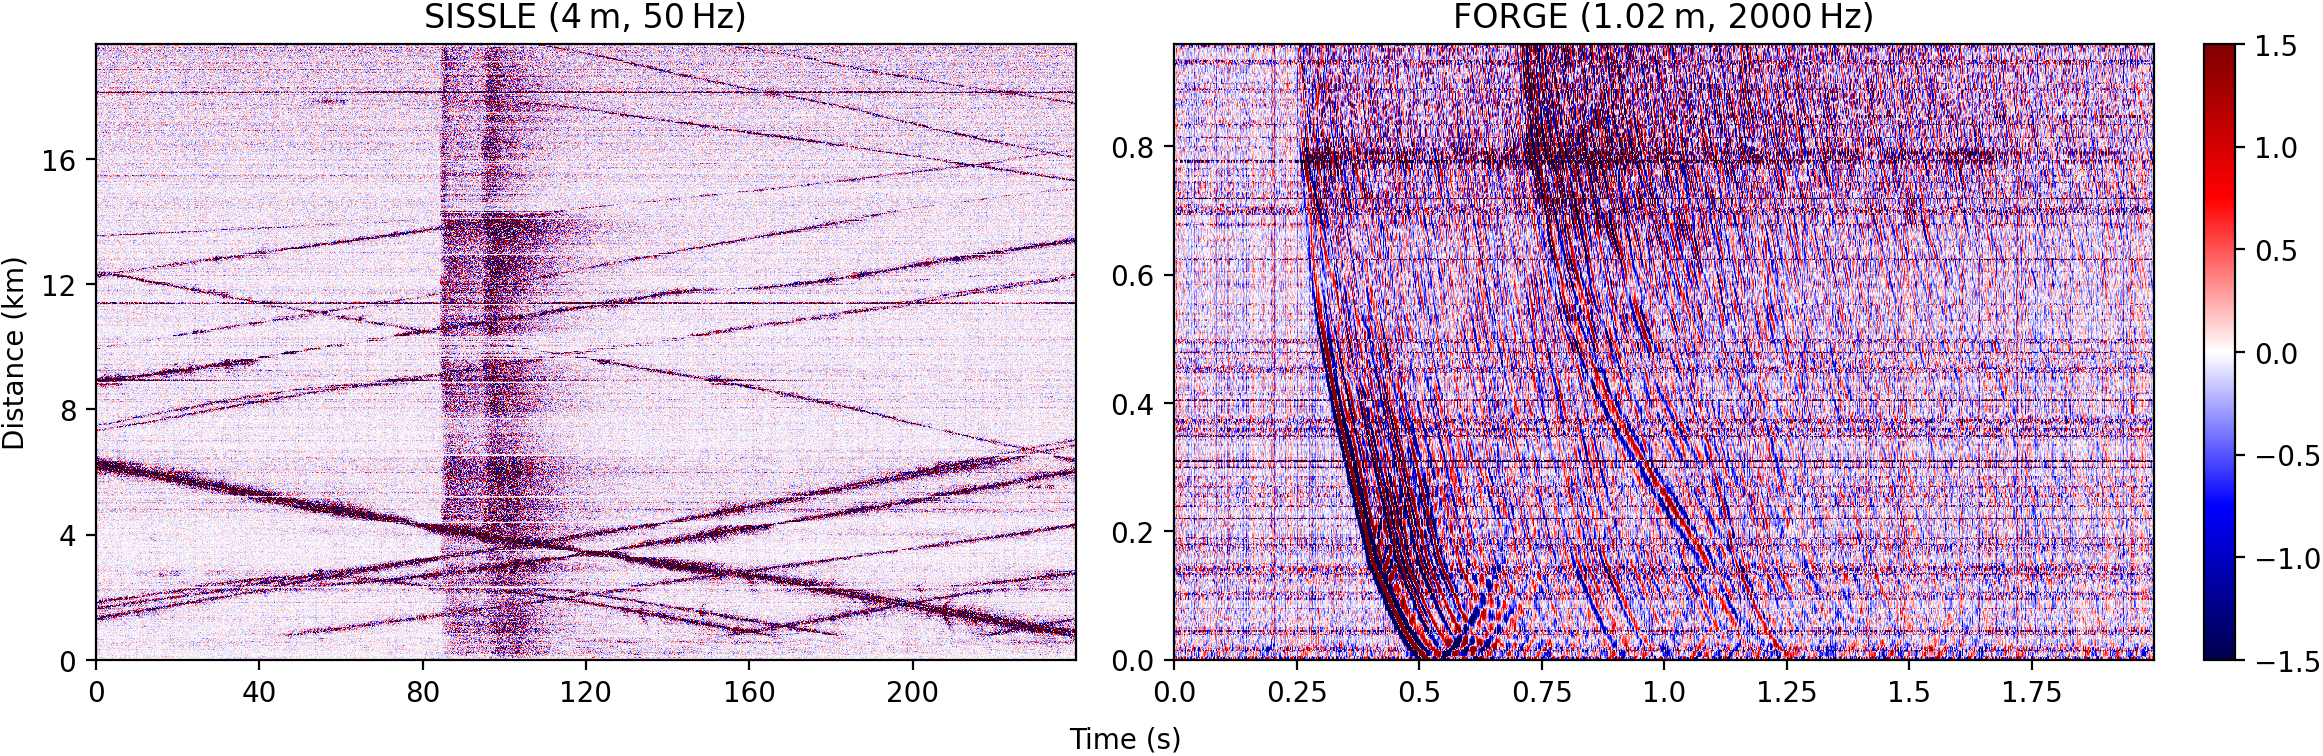
\includegraphics[width=\textwidth]{img/fig_2.2.png}
    \caption{
        Types of noise in different DAS setups.
        Both measurements capture seismic activity; however, the SISSLE data mainly suffers from traffic noise
        (the diagonal lines).
        In contrast, erratic and common mode noise (the horizontal and vertical lines,
        respectively) are most prominent in the FORGE data.
    }\label{fig:das-noise}
\end{figure}

Despite these advantages, DAS systems often suffer from much lower signal quality than conventional seismographs, as they are more sensitive to various sources of noise.
These can be divided into environmental noise and optical noise.
Environmental noise includes natural phenomena such as winds or ocean waves, but also vibrations caused by vehicular and pedestrian traffic.
Optical noise originates from various interactions between the light and the fiber.
It includes high-amplitude erratic noise and common mode noise~\cite{IDF}.\\
The actual noise characteristics of DAS data not only depend on the environment, but also the measurement parameters such as channel spacing and sample rate, as visualized in Figure~\ref{fig:das-noise} for data from the SISSLE experiment near Haast, New Zealand~\cite{SISSLE} and the FORGE site in Utah~\cite{FORGE}.

\section{Deep Learning}

Deep learning is a subfield of machine learning that utilizes deep neural networks to learn complex patterns from data. 
Over the past decade, deep learning has established itself as the state-of-the-art approach for a wide range of problems across various different fields.
% TODO such as ...

\subsection{Deep Neural Networks}

In its most basic form, a neural network consists of neurons organized in layers, where each neuron applies a linear transformation followed by a non-linear activation function.
The output of a single neuron is given by
\begin{equation}
    y = \varphi(\mathbf{w}^T\mathbf{x} + b)
\end{equation}
for an input~$\mathbf{x} \in \R^n$, a weight vector~$\mathbf{w} \in \R^n$, a bias~$b \in \R$ and an activation function~$\varphi: \R \rightarrow \R$.
The outputs of each layer are then passed as inputs to the next layer, which is why this architecture is known as a fully-connected neural network. 
The activation functions are needed in order to avoid the network collapsing into a single linear transformation. 
Therefore, a neural network can be described as a function~$f_{\theta}: \mathcal{X} \rightarrow \mathcal{Y}$ parameterized by $\theta$, where $\theta$ represents the weights and biases across all layers~\cite{DeepLearning}.

In order to optimize these parameters, a loss function~$L: \mathcal{Y} \times \mathcal{Y} \rightarrow \R$ is defined, which measures the difference between the predicted output and the target value. 
Now, the gradient of the loss function with respect to the parameters, $\nabla_\theta L = \frac{\partial L}{\partial \theta}$, represents the direction of steepest ascent.
Therefore, by moving the parameters in the opposite direction of the gradient, the loss function can be minimized.
Typically, the gradient is not calculated for a single data point or for the whole dataset, but instead for a small subset of the dataset, which is why this approach is referred to as (mini-batch) gradient descent.
Backpropagation~\cite{Backpropagation} is used to efficiently compute the gradient by making use of the chain rule, enabling fast optimization.

While traditionally neural networks only consisted of a few layers and required hand-crafted features to work effectively, advances in computing power allow modern architectures to automate feature extraction by using additional layers, hence the term \textit{deep} neural network.

\subsection{Convolutional Neural Networks}

Convolutional neural networks (CNNs)~\cite{CNN} are a specific type of neural network that learns features using kernels.
Prior to the rise of deep learning, such kernels were designed manually for various computer vision tasks, for example the Sobel kernel~\cite{Sobel} used for edge detection.
In CNNs, these kernels are automatically learned from data. In contrast to fully-connected layers, the output of a convolutional layer is obtained by convolution with one or multiple kernels, replacing the matrix multiplication.
For a kernel $\mathbf{K} \in \R^{n \times m}$, the convolution is defined as
\begin{equation}
    (\mathbf{X} \ast \mathbf{K})_{i,j} = \sum_{k=1}^{n}\sum_{l=1}^{m} X_{i+n,j+m} \cdot K_{k,l}.
\end{equation}
The output of the convolution is then passed through a non-linear activation function, just like in fully-connected layers.
CNNs provide two main advantages: First, since the weights are shared across the spatial dimensions, convolutional layers drastically reduce the number of parameters compared to fully-connected layers. 
Second, convolutions are translationally equivariant, meaning that local patterns in the input can be recognized regardless of their position, which makes CNNs very suitable for image data~\cite{DeepLearning}.

\subsection{Normalization}

\begin{figure}
    \centering
    \tdplotsetmaincoords{60}{-45}

    \newcommand{\cube}[2]{
        % background
        \fill[gray!10, opacity=0.5] (0,0,#1) -- (#1,0,#1) -- (#1,#1,#1) -- (0,#1,#1) -- cycle;
        \fill[gray!10, opacity=0.5] (0,0,0) -- (#1,0,0) -- (#1,0,#1) -- (0,0,#1) -- cycle;
        \fill[gray!10, opacity=0.5] (0,0,0) -- (0,#1,0) -- (0,#1,#1) -- (0,0,#1) -- cycle;
    
        % edges
        \draw[thick] (0,0,0) -- (0,0,#1);
        \draw[thick] (0,#1,#1) -- (0,#1,0) -- (0,0,0) -- (#1,0,0) -- (#1,0,#1);
        \draw[thick] (0,#1,#1) -- (0,0,#1) -- (#1,0,#1) -- (#1,#1,#1) -- cycle;
    
        % grid
        \foreach \i in {1,2,...,\numexpr#1-1\relax} {
            \draw[very thin] (0,\i,0) -- (0,\i,#1);
            \draw[very thin] (0,0,\i) -- (0,#1,\i);
    
            \draw[very thin] (\i,0,0) -- (\i,0,#1);
            \draw[very thin] (0,0,\i) -- (#1,0,\i);
    
            \draw[very thin] (\i,0,#1) -- (\i,#1,#1);
            \draw[very thin] (0,\i,#1) -- (#1,\i,#1);
        }
    
        % labels
        \node[rotate=90] at (0,#1,#1/2) [above] {$H,W$};
        \node at (0,#1/2,0) [below left] {$C$};
        \node at (#1/2,0,0) [below right] {$N$};
    
        % name
        \node at (#1,#1,#1+1) {#2};
    }

    \def\a{4}
    \begin{tikzpicture}[tdplot_main_coords, line join=round, scale=0.5]
        \fill[Maroon] (0,0,0) -- (\a,0,0) -- (\a,0,\a) -- (0,0,\a) -- cycle;
        \fill[Maroon] (0,0,0) -- (0,1,0) -- (0,1,\a) -- (0,0,\a) -- cycle;
        \fill[Maroon] (0,0,\a) -- (\a,0,\a) -- (\a,1,\a) -- (0,1,\a) -- cycle;

        \cube{\a}{Batch Norm}
    \end{tikzpicture}
    \hfill
    \begin{tikzpicture}[tdplot_main_coords, line join=round, scale=0.5]
        \fill[Maroon] (0,0,0) -- (0,\a,0) -- (0,\a,\a) -- (0,0,\a) -- cycle;
        \fill[Maroon] (0,0,0) -- (1,0,0) -- (1,0,\a) -- (0,0,\a) -- cycle;
        \fill[Maroon] (0,0,\a) -- (0,\a,\a) -- (1,\a,\a) -- (1,0,\a) -- cycle;

        \cube{\a}{Layer Norm}
    \end{tikzpicture}
    \hfill
    \begin{tikzpicture}[tdplot_main_coords, line join=round, scale=0.5]
        \fill[Maroon] (0,0,0) -- (0,1,0) -- (0,1,\a) -- (0,0,\a) -- cycle;
        \fill[Maroon] (0,0,0) -- (1,0,0) -- (1,0,\a) -- (0,0,\a) -- cycle;
        \fill[Maroon] (0,0,\a) -- (0,1,\a) -- (1,1,\a) -- (1,0,\a) -- cycle;

        \cube{\a}{Instance Norm}
    \end{tikzpicture}
    \hfill
    \begin{tikzpicture}[tdplot_main_coords, line join=round, scale=0.5]
        \fill[Maroon] (0,0,0) -- (0,\a/2,0) -- (0,\a/2,\a) -- (0,0,\a) -- cycle;
        \fill[Maroon] (0,0,0) -- (1,0,0) -- (1,0,\a) -- (0,0,\a) -- cycle;
        \fill[Maroon] (0,0,\a) -- (0,\a/2,\a) -- (1,\a/2,\a) -- (1,0,\a) -- cycle;

        \cube{\a}{Group Norm}
    \end{tikzpicture}

    \caption{
        Different normalization techniques. $N$ is the batch dimension, $C$ is the channel dimension and $H$ and $W$ are
        the spatial dimensions of a 4D tensor. The input is normalized across the dimensions highlighted in red.
        Figure adapted from~\cite{GroupNorm}.
    }\label{fig:normalization}
\end{figure}

During the training process, the inputs of each layer change with each iteration as the parameters are optimized.
That slows down the training because now each layer has to adapt to the new distribution of its inputs. This process is often referred to as internal covariate shift.
To counteract this issue, Ioffe~et al.\ proposed Batch Normalization (BN)~\cite{BatchNorm}.
The idea behind BN is to normalize the inputs across the whole mini-batch and their spatial dimensions.
The normalized input for a channel $i$ is given by
\begin{equation}
    \hat{x}^{(i)} = \frac{x^{(i)} - \mu^{(i)}}{\sigma^{(i)}},
\end{equation} 
where $\mu^{(i)}$ and $\sigma^{(i)}$ are the per-channel mean and standard deviation of the mini-batch, respectively.  
In order to allow the model to learn the identity if that were the optimal transformation, two additional learnable parameters, $\gamma$ and $\beta$, are introduced. The output of the BN layer is then defined as
\begin{equation}
    y^{(i)} = \gamma^{(i)}\hat{x}^{(i)} + \beta^{(i)}.
\end{equation}
Since there are no batch statistics available at inference time, BN keeps track of the running mean and variance during training and uses these values for normalization.
While BN is widely used, there exist various similar normalization techniques~\cite{LayerNorm, InstanceNorm, GroupNorm} mainly differing in the dimensions across which they are applied.
A selection of them is visualized in Figure~\ref{fig:normalization}.


\subsection{Attention Mechanisms}

In neural networks, some input features are typically more important than others.
An attention mechanism helps the network to focus on (\textit{attend to}) the most relevant parts of the input, rather than processing all inputs equally.
This works by dynamically reweighting the features based on their importance~\cite{Attention}.
While attention is often associated with natural language processing (NLP), especially since the introduction of the Transformer architecture~\cite{Transformer} where it is the underlying key principle, it also has applications beyond NLP.\@
In computer vision, for example, it can help CNNs by reweighting feature channels~\cite{SqueezeExcite} or highlighting important spatial regions.
% TODO add details

\section{Fourier Transform}
% TODO add fourier?
